%========================================================================
% Modelo para elaboracao de textos academicos: TCC, dissertacoes e teses
% Elaborado pelo GISIS - Grupo de Imageamento Sismico e Inversao Sismica.
%========================================================================
\chapter{Resultados}
\label{ch:resultados}

Neste capítulo, são apresentados os resultados da comparação entre os métodos de \citeonline{podvin1991finite}, \citeonline{jeong2008fast} e \citeonline{noble2014accurate} em termos de precisão no cálculo dos tempos de trânsito, desempenho computacional e recuperação dos modelos por inversão tomográfica. 

\section{Experimentos comparativos de modelagem}

Como relatado no capítulo anterior, experimentos com modelo homogêneo, de refração e complexo são explorados. A aplicação com modelo homogêneo replica o experimento realizado no trabalho de \citeonline{cai2023improved}, onde a inovação em precisão foi desenvolvida para o \textit{Fast Iterative Method}. A aplicação com modelo de duas camadas replica o experimento realizado no Simpósio Brasileiro de Geofísica de 2022. E a aplicação em modelo complexo mostra como os tempos de trânsito se comportam na presença de altos contrastes de velocidade e qual o tempo de execução para cada método no modelo mais realístico.    

\subsection{Aplicação em modelo homogêneo}

A Tabela \ref{table_homog} mostra os tempos de execução, o erro médio e o erro máximo para cada formulação. Os resultados gerados utilizando a implementação de \citeonline{cai2023improved} foram executados no mesmo ambiente que os demais métodos, devido a disponibilização do código publicamente.   

\begin{table}[H]
	\caption{Tempo de execução, erro médio e máximo em relação a equação analítica para meio homogêneo. Aplicação dos métodos utilizados relacionando com os resultados do experimento de \citeonline{cai2023improved}.}
	\begin{tabular}{r|ccc}
		\multicolumn{1}{c|}{} & Tempo {[}s{]} & Erro médio {[}s{]} & Erro máximo {[}s{]} \\ \hline
		\citeonline{podvin1991finite} & 0,9661        & 0,000273           & 0,000762            \\ \hline
		\citeonline{jeong2008fast}    & 0,6082        & 0,000837           & 0,001323            \\ \hline
		\citeonline{noble2014accurate}& 0,8085        & 0,000037           & 0,000069            \\ \hline
		\citeonline{cai2023improved}  & 1,9312        & 0,000196           & 0,000282           
	\end{tabular}
	\label{table_homog}
\end{table}

\subsection{Aplicação em modelo de refração}

A Figura \ref{fig:resultsNumericalComparison} mostra todo o estudo de precisão com os tempos calculados da fonte para os receptores e dos receptores para a fonte (reciprocidade). As cores indicam os métodos, sendo o azul para a formulação de \citeonline{podvin1991finite}, o amarelo para a formulação de \citeonline{jeong2008fast} e o verde para a formulação de \citeonline{noble2014accurate}. Os estilos de linha representam o parâmetro de discretização, então, as linhas sólidas representam o modelo de 25 m, as linhas tracejadas, o de 50 m, e as linhas com ponto e traço, o de 100 m. A Figura \ref{fig:resultsNumericalComparison}a mostra a configuração de todos os métodos para o tiro central, sendo o tempo analítico a linha sólida de cor preta. As Figuras \ref{fig:resultsNumericalComparison}c, \ref{fig:resultsNumericalComparison}e e \ref{fig:resultsNumericalComparison}g mostram a ordem do erro para cada método e as Figuras \ref{fig:resultsNumericalComparison}d, \ref{fig:resultsNumericalComparison}f e \ref{fig:resultsNumericalComparison}h mostram as diferenças entre o tempo direto e recíproco para cada método utilizando o modelo de 25 m.  

\begin{figure}[H]
	\centering
	\subfloat[]{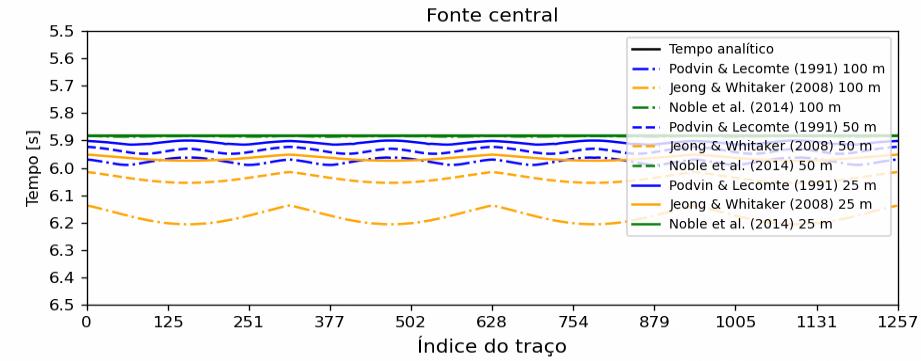
\includegraphics[width=8cm,height=3.5cm]{Imgs/RevisaoBibliografica/precision_direct.png}\label{fig:rnca}}
	\subfloat[]{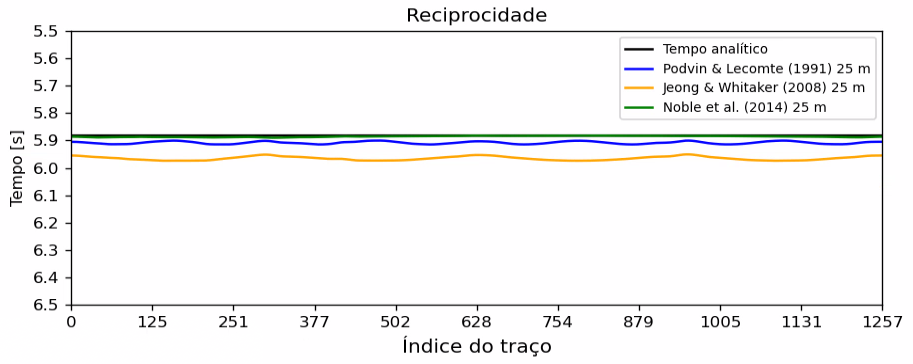
\includegraphics[width=8cm,height=3.5cm]{Imgs/RevisaoBibliografica/reciprocity.png}\label{fig:rncb}}
	
	\subfloat[]{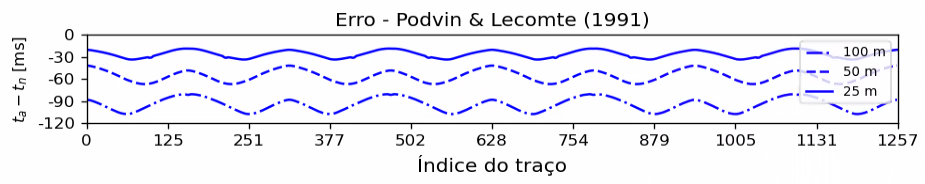
\includegraphics[width=8cm,height=1.5cm]{Imgs/RevisaoBibliografica/error_pod_direct.png}\label{fig:rncc}}
	\subfloat[]{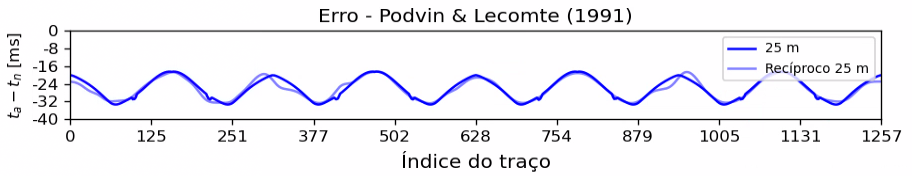
\includegraphics[width=8cm,height=1.5cm]{Imgs/RevisaoBibliografica/error_pod_reciprocity.png}\label{fig:rncd}}
	
	\subfloat[]{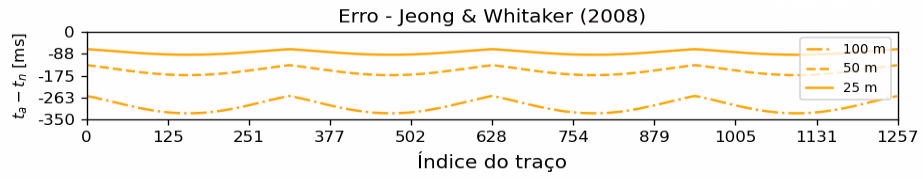
\includegraphics[width=8cm,height=1.5cm]{Imgs/RevisaoBibliografica/error_fim_direct.png}\label{fig:rnce}}
	\subfloat[]{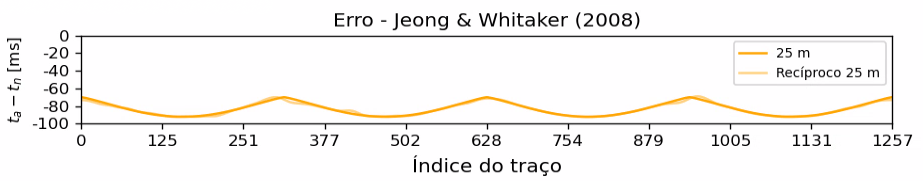
\includegraphics[width=8cm,height=1.5cm]{Imgs/RevisaoBibliografica/error_fim_reciprocity.png}\label{fig:rncf}}
	
	\subfloat[]{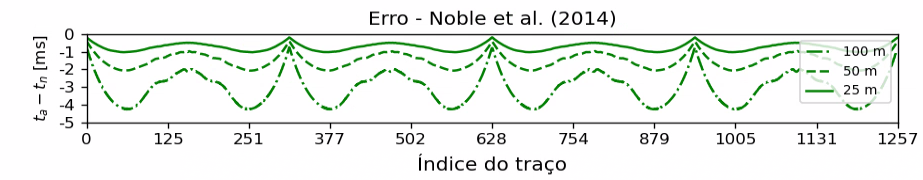
\includegraphics[width=8cm,height=1.5cm]{Imgs/RevisaoBibliografica/error_fsm_direct.png}\label{fig:rncg}}
	\subfloat[]{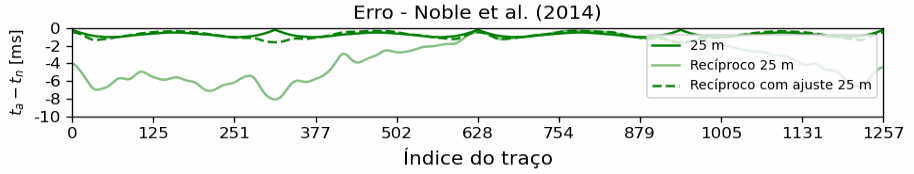
\includegraphics[width=8cm,height=1.5cm]{Imgs/RevisaoBibliografica/error_fsm_reciprocity.png}\label{fig:rnch}}
	
	\caption{(a) Mapeamento das chegadas para os métodos numéricos testados para os espaçamentos estudados. (b) Estudo de reciprocidade utilizando o espaçamento de 25 m. (c) Escala do erro para as chegadas em diferentes espaçamentos e (d) tempo direto e recíproco da formulação de \citeonline{podvin1991finite}. (e) Escala do erro e (f) reciprocidade para o método de \citeonline{jeong2008fast}. (g) Escala do erro e (h) reciprocidade para o método de \citeonline{noble2014accurate}.}
	\label{fig:resultsNumericalComparison}
\end{figure}

A superioridade de precisão do método \citeonline{noble2014accurate} pode ser identificada, porém no estudo de reciprocidade a inicialização causou instabilidade, como mostrado na Figura \ref{fig:resultsNumericalComparison}h. Para iniciar o cálculo dos tempos de trânsito, todo o volume é inicializado com um valor tendendo ao infinito e somente os pontos vizinhos da fonte são inicializados com o tempo analítico para velocidade constante. O algoritmo original de \citeonline{noble2014accurate} inicializa analiticamente somente os pontos do primeiro octante, porém o estudo de reciprocidade mostrou que a inicialização deve ser feita para os pontos vizinhos em todas as direções.  

A Tabela \ref{table_refModel} mostra, para cada método testado, seus respectivos resultados de tempo de execução. A análise de reciprocidade foi crucial para verificar extravasamentos de memória quando aplicadas múltiplas posições de tiro. A validação em aplicações de imageamento sísmico também pode ser observada a partir do estudo de reciprocidade, pois o tempo de execução importa na geração de resultados.  

\begin{table}[H]
	\caption{Tempo de execução para cada discretização e reciprocidade para o modelo de 25 m.}
	\begin{tabular}{r|cccc}
		& 100 m    & 50 m     & 25 m     & Reciprocidade \\ \hline
		\citeonline{podvin1991finite}   & 0,0676 s & 0,3141 s & 3,5324 s & 7896,2 s        \\ \hline
		\citeonline{jeong2008fast} & 0,0491 s & 0,0987 s & 0,6261 s & 921,8 s              \\ \hline
		\citeonline{noble2014accurate} & 0,1042 s & 0,2286 s & 0,8284 s & 1382,5 s          \\
	\end{tabular}
	\label{table_refModel}
\end{table}

\subsection{Aplicação em modelo complexo}

A Figura \ref{fig:result_overthrust} mostra os resultados gerados a partir do esquema de modelagem com geometria circular aplicado no modelo SEG/EAGE \textit{Overthrust}. Novamente as cores da figura indicam cada método, sendo a cor azul para a formulação de \citeonline{podvin1991finite}, laranja para \citeonline{jeong2008fast} e verde para a formulação de \citeonline{noble2014accurate}. As Figuras \ref{fig:result_overthrust}b, \ref{fig:result_overthrust}c e \ref{fig:result_overthrust}d são ampliações do sismograma de primeira chegada. Como a equação eikonal é uma aproximação da equação da onda para altas frequências, espera-se que os detalhes do modelo sejam identificados no dado, então, as janelas amplificadoras facilitam a identificação desses aspectos.    

\begin{table}[H]
	\caption{Tempo de execução para a aplicação dos métodos no modelo complexo.}
	\begin{tabular}{r|c}
		& Tempo de execução \\ \hline
		\citeonline{podvin1991finite} & 11,7128 s  \\ \hline
		\citeonline{jeong2008fast} & 2,5595 s      \\ \hline
		\citeonline{noble2014accurate} & 3,4746 s         
	\end{tabular}
	\label{table_overthrust}
\end{table}

A Tabela \ref{table_overthrust} mostra os tempos de execução para cada método utilizando o modelo complexo em geometria circular aplicando somente um tiro no centro do modelo. A superioridade de performance é atribuída ao método de \citeonline{jeong2008fast}, porém essa metodologia possui atrasos severos em relação aos tempos de trânsito calculados comparado à equação analítica e aos demais métodos testados.

\begin{figure}[H]
	\centering
	\subfloat[]{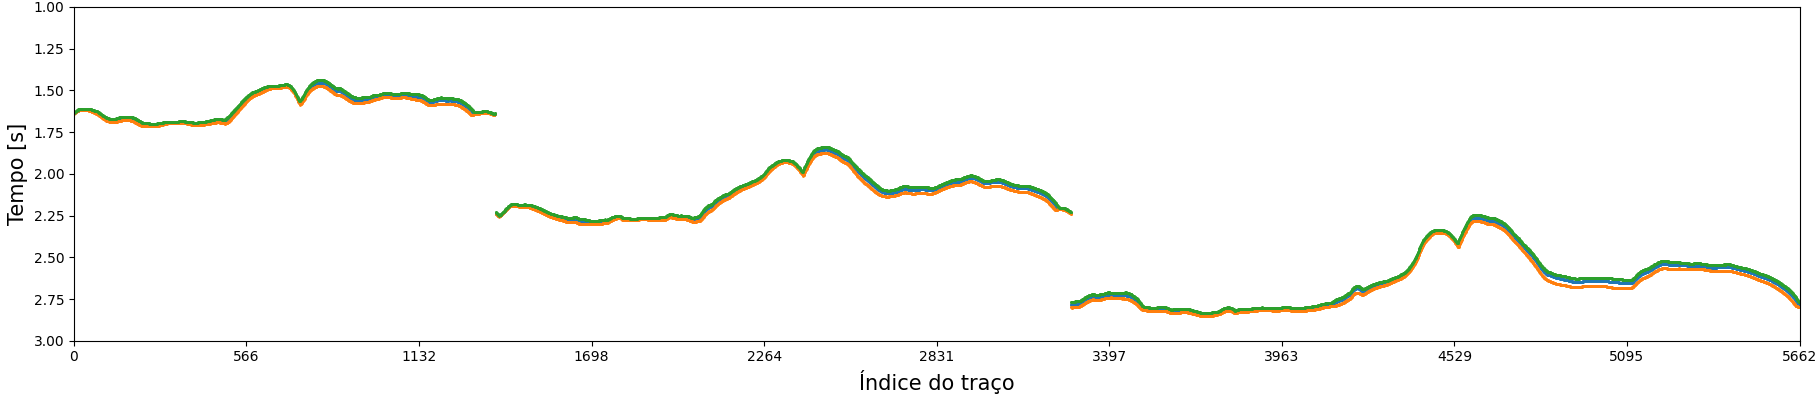
\includegraphics[height=4cm,width=16cm]{Imgs/Resultados/complex_model_full.png}} \\
	\subfloat[]{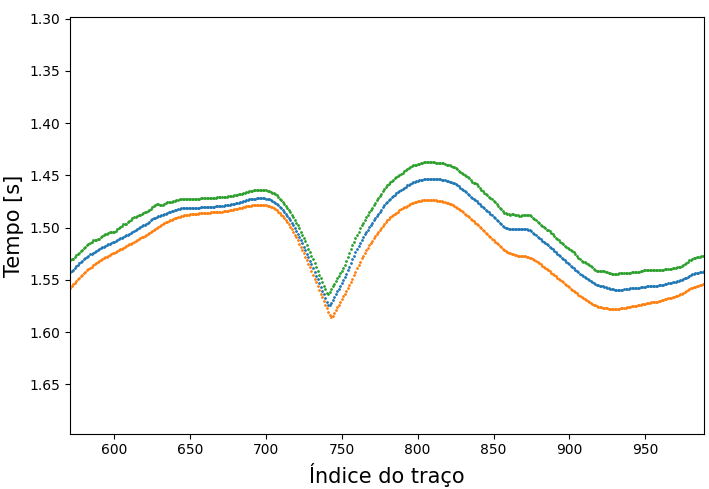
\includegraphics[height=3cm,width=5cm]{Imgs/Resultados/complex_w1.png}} \hfill
	\subfloat[]{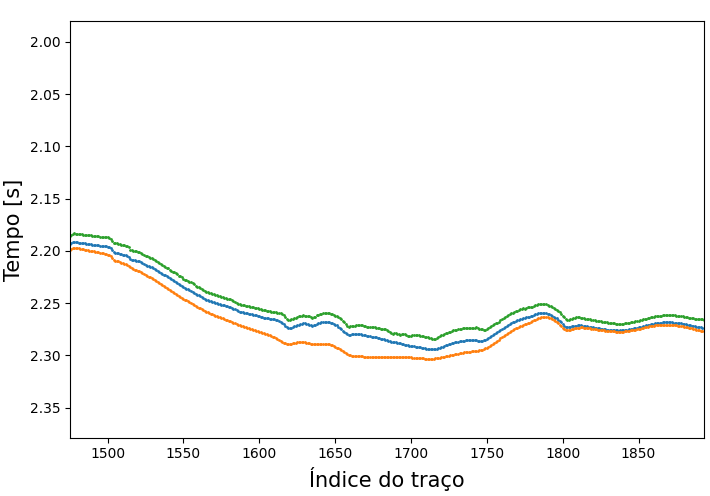
\includegraphics[height=3cm,width=5cm]{Imgs/Resultados/complex_w2.png}} \hfill
	\subfloat[]{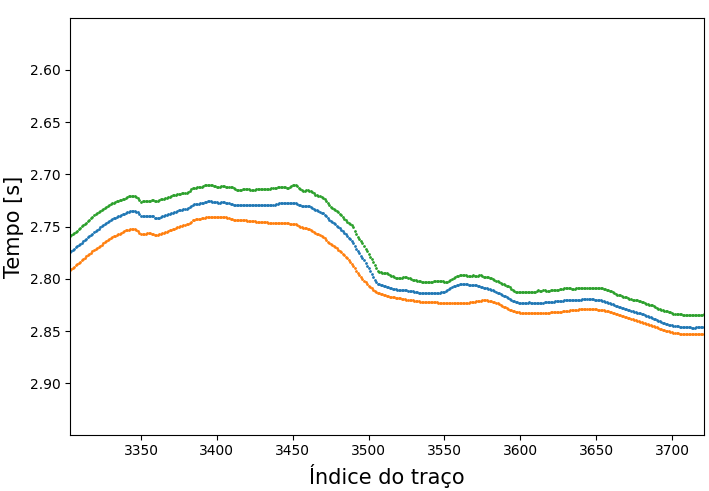
\includegraphics[height=3cm,width=5cm]{Imgs/Resultados/complex_w3.png}}
	\caption{Tempos de trânsito calculados para cada método para o esquema de modelo complexo. As cores representam cada formulação, sendo a cor azul para \citeonline{podvin1991finite}, laranja para \citeonline{jeong2008fast} e verde para \citeonline{noble2014accurate}.(a) Tempos para todos os traços da geometria circular, (b), (c) e (d) são janelas amplificadoras para mostrar os atrasos dos tempos de trânsito.}
	\label{fig:result_overthrust}	
\end{figure}

\section{Experimento tomográfico}

Basicamente, os resultados gerados pelo processo tomográfico não linear são os modelos da última iteração e as curvas de convergência indicando a diminuição da função objetivo minimizando a diferença entre o dado observado e calculado. O esquema realizado se divide em duas etapas, sendo a primeira uma inversão utilizando um modelo de malha esparsa e a segunda utilizando o modelo resultante da inversão anterior aplicando uma malha refinada. A Figura \ref{fig:convergencia} mostra a curva de convergência para as duas etapas de inversão, sendo que até a quinta iteração o processo aplicado foi utilizando a malha esparsa e as demais iterações para malha refinada, totalizando dez iterações na tentativa de realçar detalhes no modelo de velocidade.   

\begin{figure}[H]
	\centering
	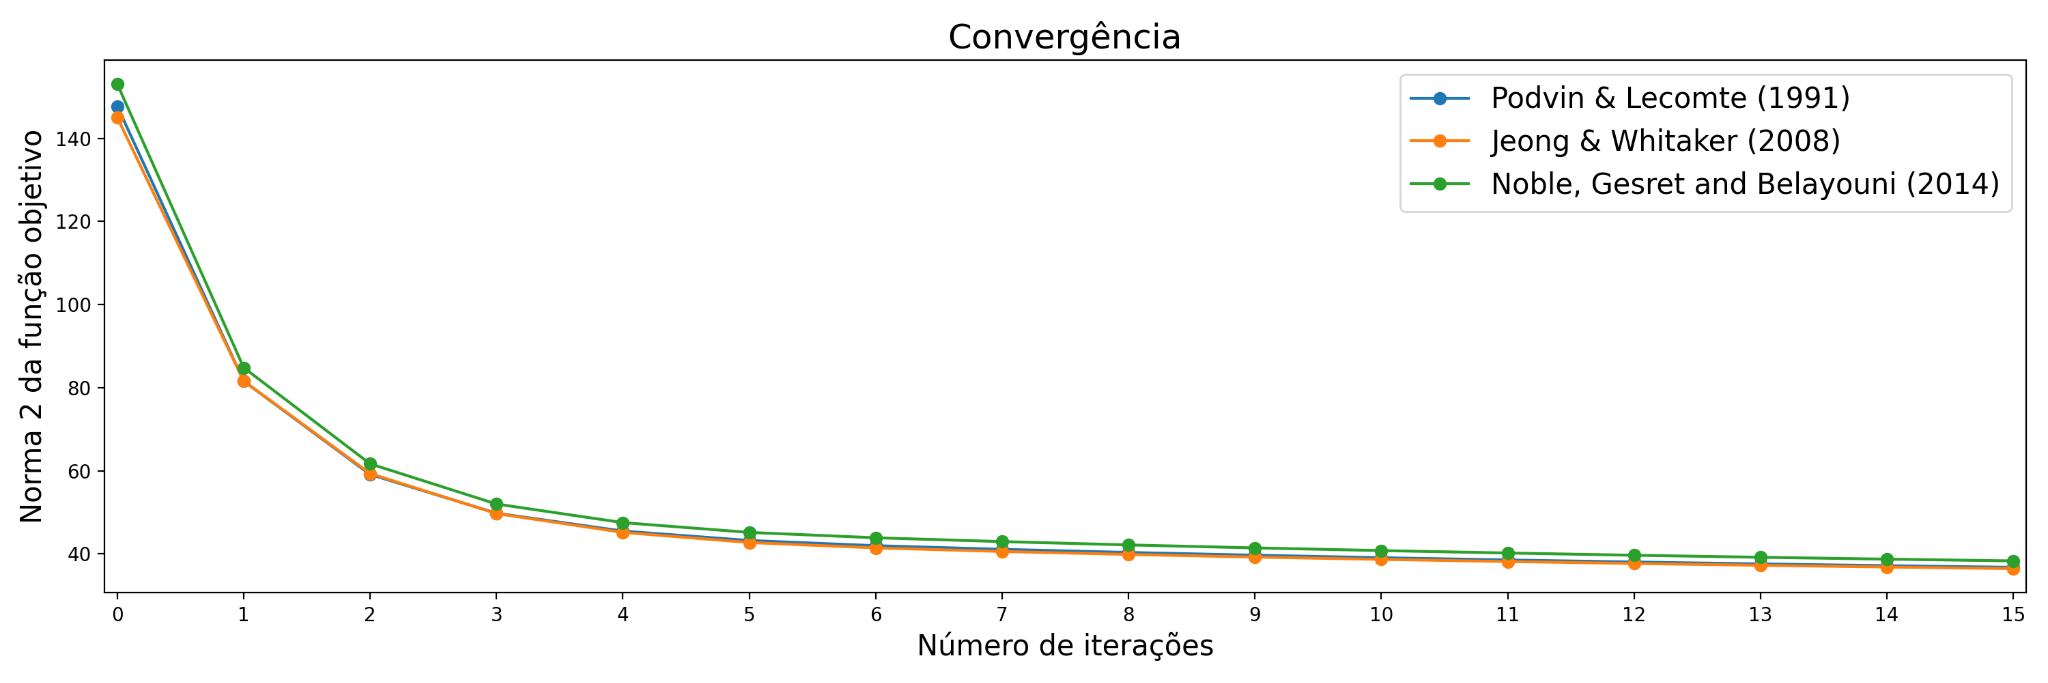
\includegraphics[width=16cm,height=6cm]{Imgs/Resultados/convergencia.png}
	\caption{Mapa de convergência tomográfica para os métodos estudados. Iterações entre 0 e 5 a malha esparsa foi aplicada no processo de inversão. Iterações entre 6 e 15 a malha refinada foi utilizada na tomografia.}
	\label{fig:convergencia}	
\end{figure}

Os modelos foram limitados e o descarte das amostras nas extremidades do modelo foi considerado no momento da otimização. Esse descarte ocorreu pois os raios não iluminavam essas regiões e assim uma instabilidade na solução do sistema linear era registrada. A eliminação das amostras ocorreu em um espaçamento de 200 m nas laterais do modelo. A inversão também não considerou atualizações na camada de água, somente a partir de uma profundidade fixa de 200 m. O horizonte do fundo marinho do modelo de referência tem profundidade mínima de 200 m, ou seja, a profundidade do horizonte está inteiramente contida no domínio da inversão.     

\subsection{Inversão com malha esparsa}

Os modelos recuperados utilizando a inversão com malha esparsa podem ser visualizados nas Figuras \ref{fig:pod_sparse}, \ref{fig:fim_sparse} e \ref{fig:fsm_sparse}, sendo que os métodos de \citeonline{podvin1991finite}, \citeonline{jeong2008fast} e \citeonline{noble2014accurate} foram considerados, respectivamente, na resolução do problema direto. Todos os modelos apresentaram aspectos suaves pelo estilo de regularização empregado e pela suavização gaussiana empregada a cada iteração. A segunda condição de suavização imposta se concretizou na tentativa de reduzir artefatos nos modelos recuperados. A suavização gaussiana foi aplicada na variação da vagarosidade recuperada após a resolução do sistema linear com uma janela de cinco amostras e desvio padrão $\sigma = 2$. Nas imagens de resultado, o descarte de pontos nas extremidades do modelo fica nítido pois nessas regiões o modelo inicial foi completamente conservado.

\begin{figure}[H]
	\centering
	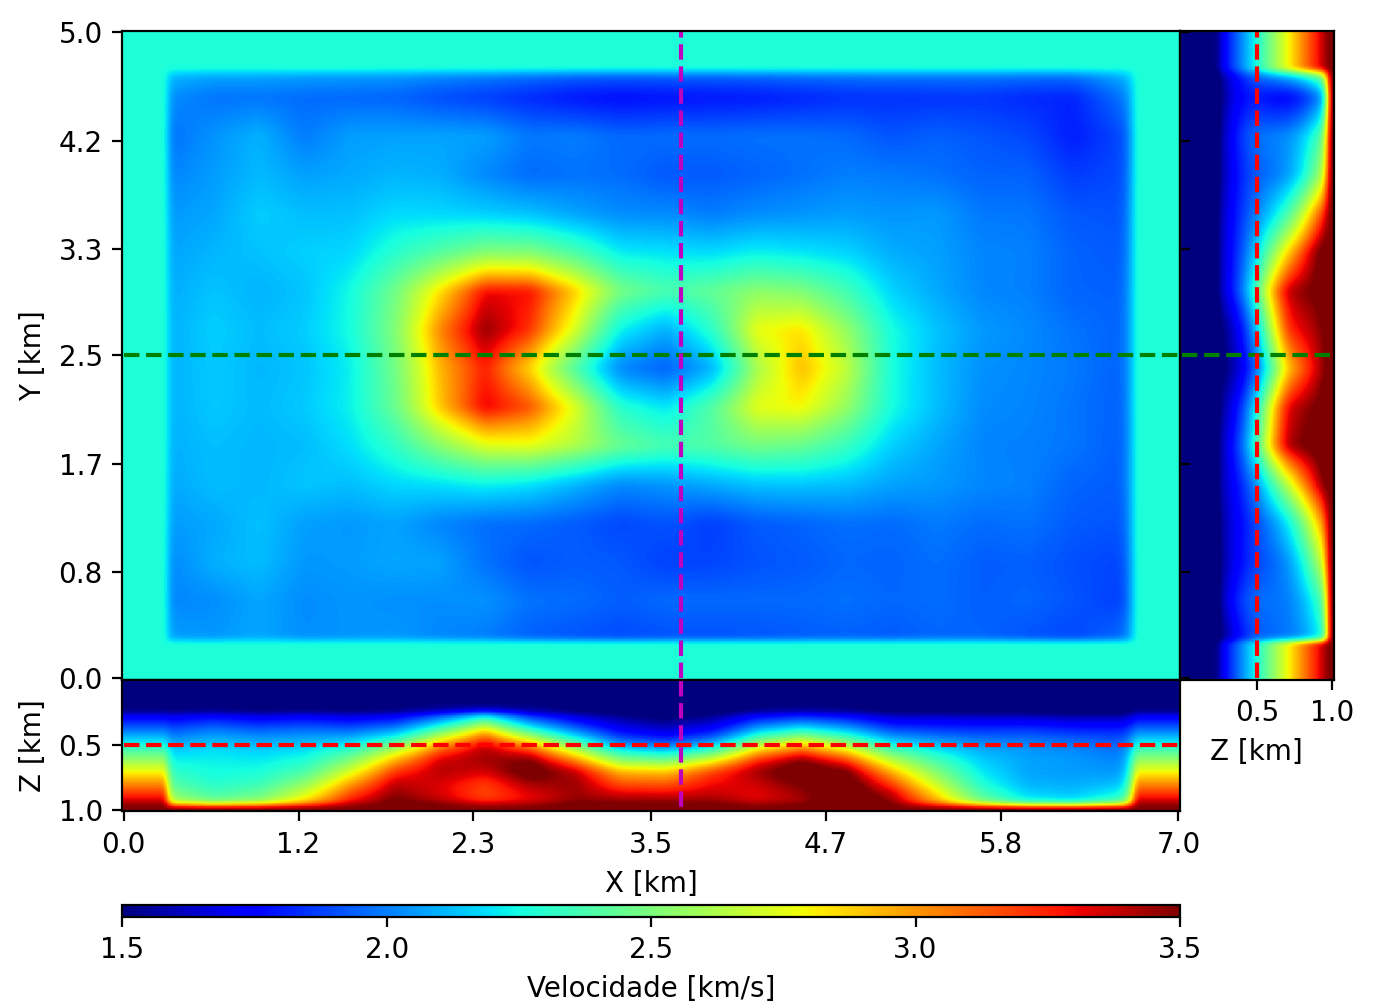
\includegraphics[width=12cm,height=9cm]{Imgs/Resultados/pod_sparse.png}
	\caption{Modelo obtido utilizando o método clássico em malha esparsa.}
	\label{fig:pod_sparse}	
\end{figure}

\begin{figure}[H]
	\centering
	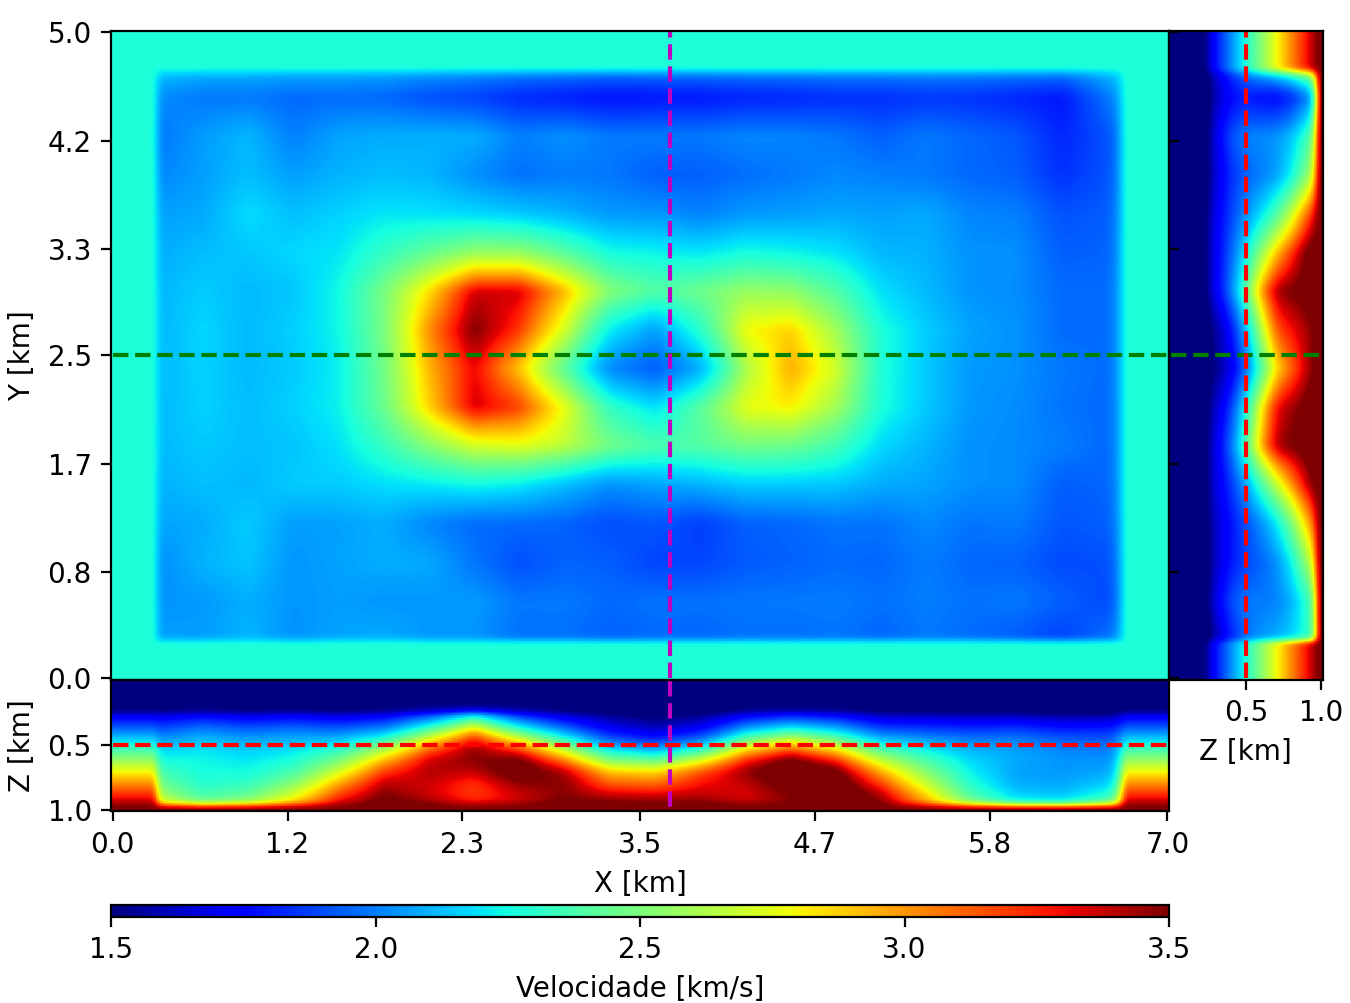
\includegraphics[width=12cm,height=9cm]{Imgs/Resultados/fim_sparse.png}
	\caption{Modelo obtido utilizando o \textit{Fast Iterative Method} em malha esparsa.}
	\label{fig:fim_sparse}	
\end{figure}

A redução do tamanho da malha pode ser um estabilizador do problema tomográfico, já que mais raios iluminam as células tornando o problema inverso melhor determinado. A suavidade do modelo já era esperada pois os artifícios de interpolação trilinear da variação do modelo de vagarosidade recuperado a cada iteração prejudica a conservação de altos contrastes.     

\begin{figure}[H]
	\centering
	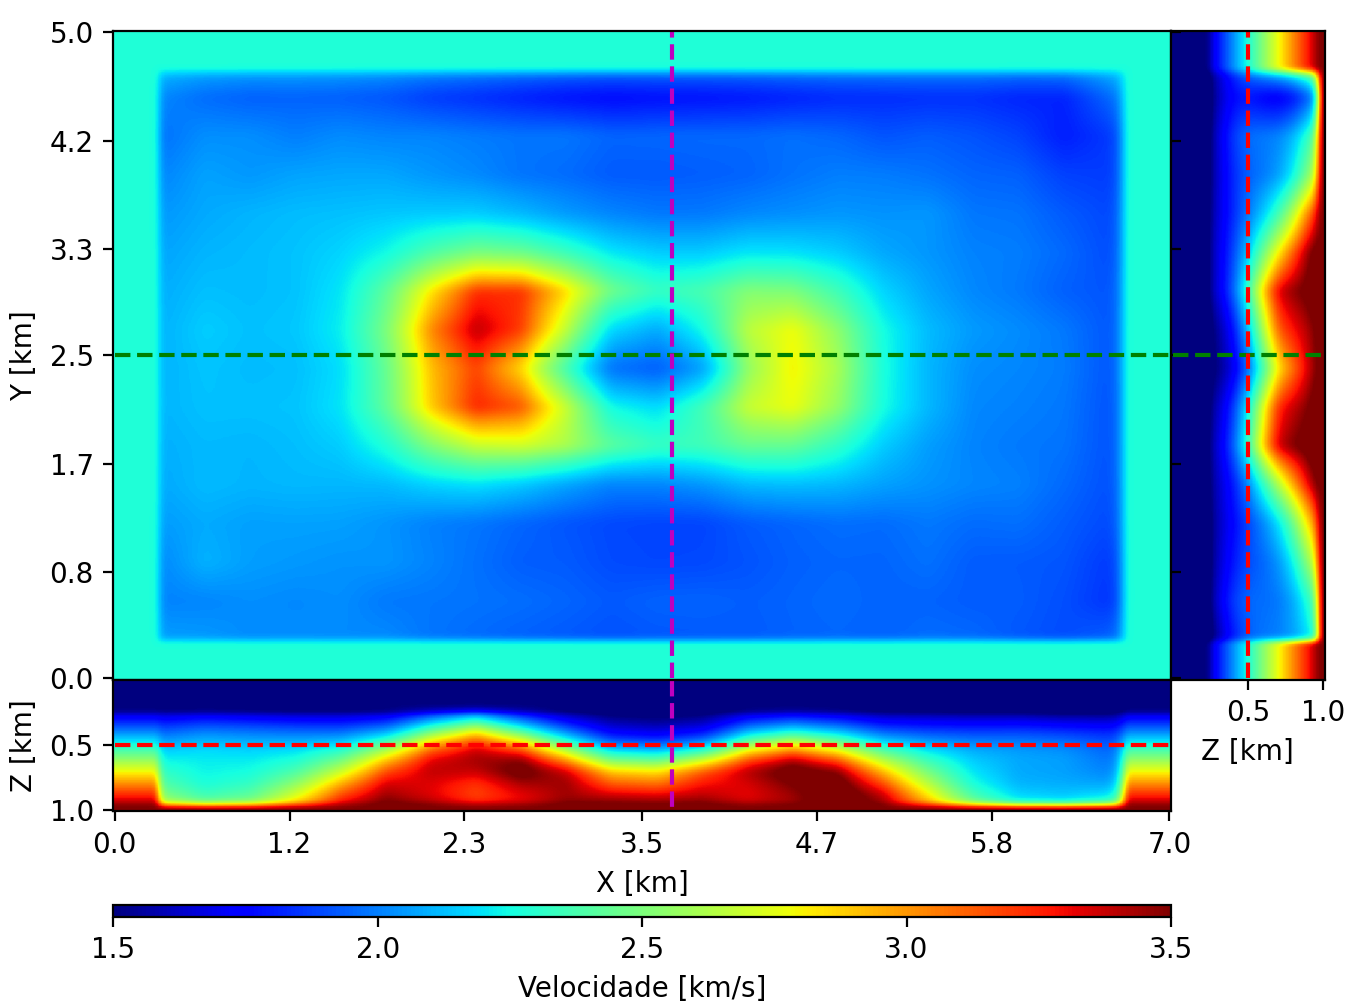
\includegraphics[width=12cm,height=9cm]{Imgs/Resultados/fsm_sparse.png}
	\caption{Modelo obtido utilizando o \textit{Fast Sweeping Method} em malha esparsa.}
	\label{fig:fsm_sparse}	
\end{figure}

\subsection*{Inversão com malha refinada}

Os resultados após dez iterações com malha refinada utilizando como modelo inicial os resultados anteriores obtidos com a malha esparsa estão ilustrados nas Figuras \ref{fig:pod_refined}, \ref{fig:fim_refined} e \ref{fig:fsm_refined}, com a mesma sequência de métodos utilizada no resultado de malha esparsa.

\begin{figure}[H]
	\centering
	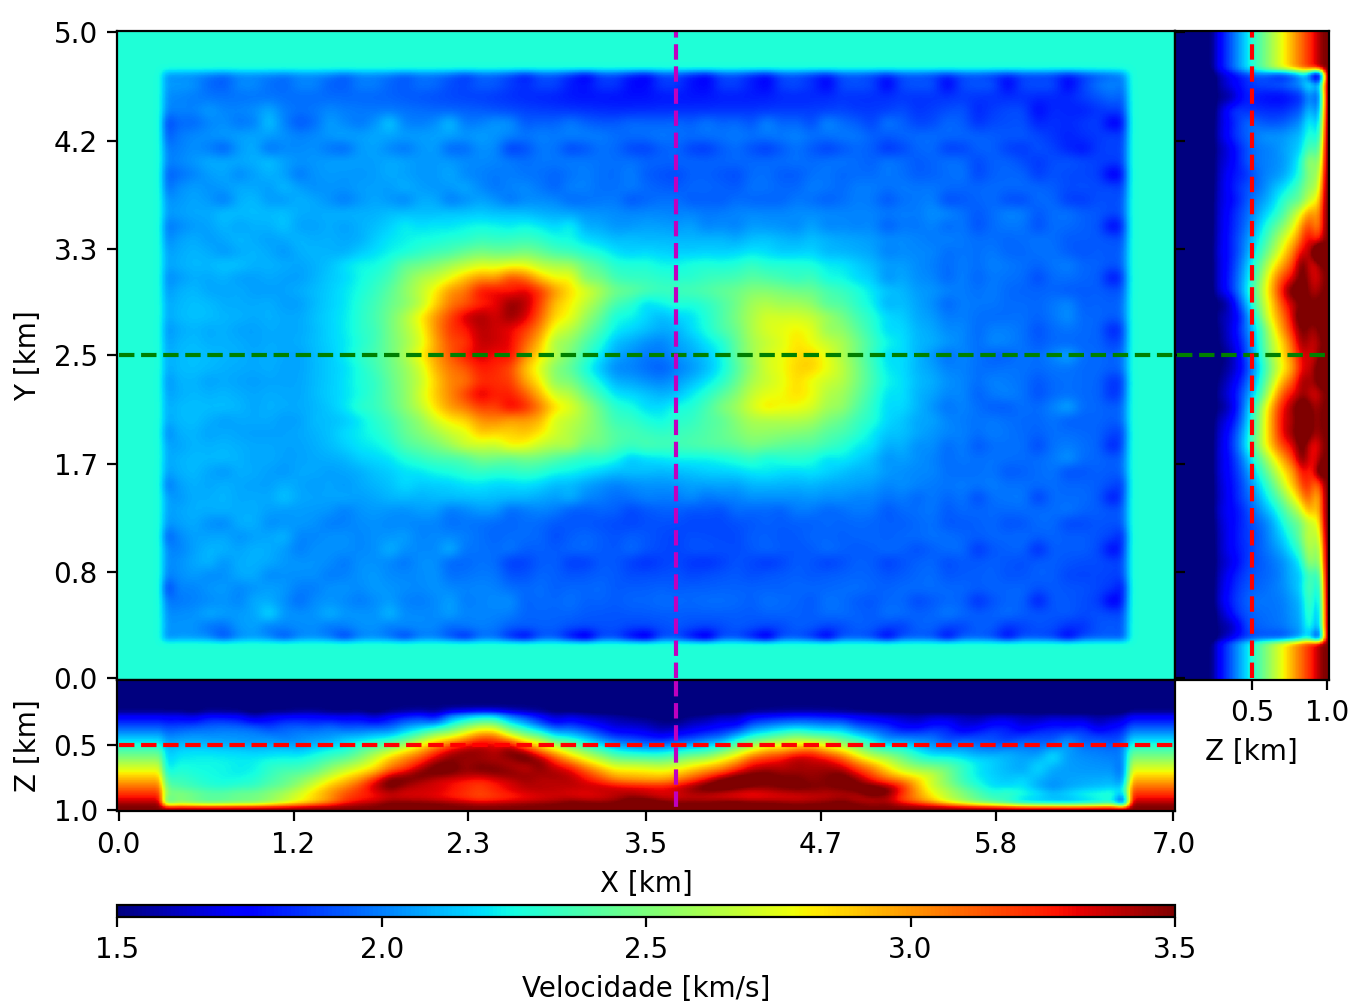
\includegraphics[width=12cm,height=9cm]{Imgs/Resultados/pod_refined.png}
	\caption{Modelo recuperado utilizando o método clássico em malha refinada.}
	\label{fig:pod_refined}	
\end{figure}

Para efeitos de realce dos detalhes no modelo de velocidade recuperado, a suavização gaussiana iterativa foi desativada no processo tomográfico. Portanto, nota-se um aumento dos artefatos de inversão causados pela distância entre as posições de receptores, já que a simulação utilizou o princípio da reciprocidade.  

\begin{figure}[H]
	\centering
	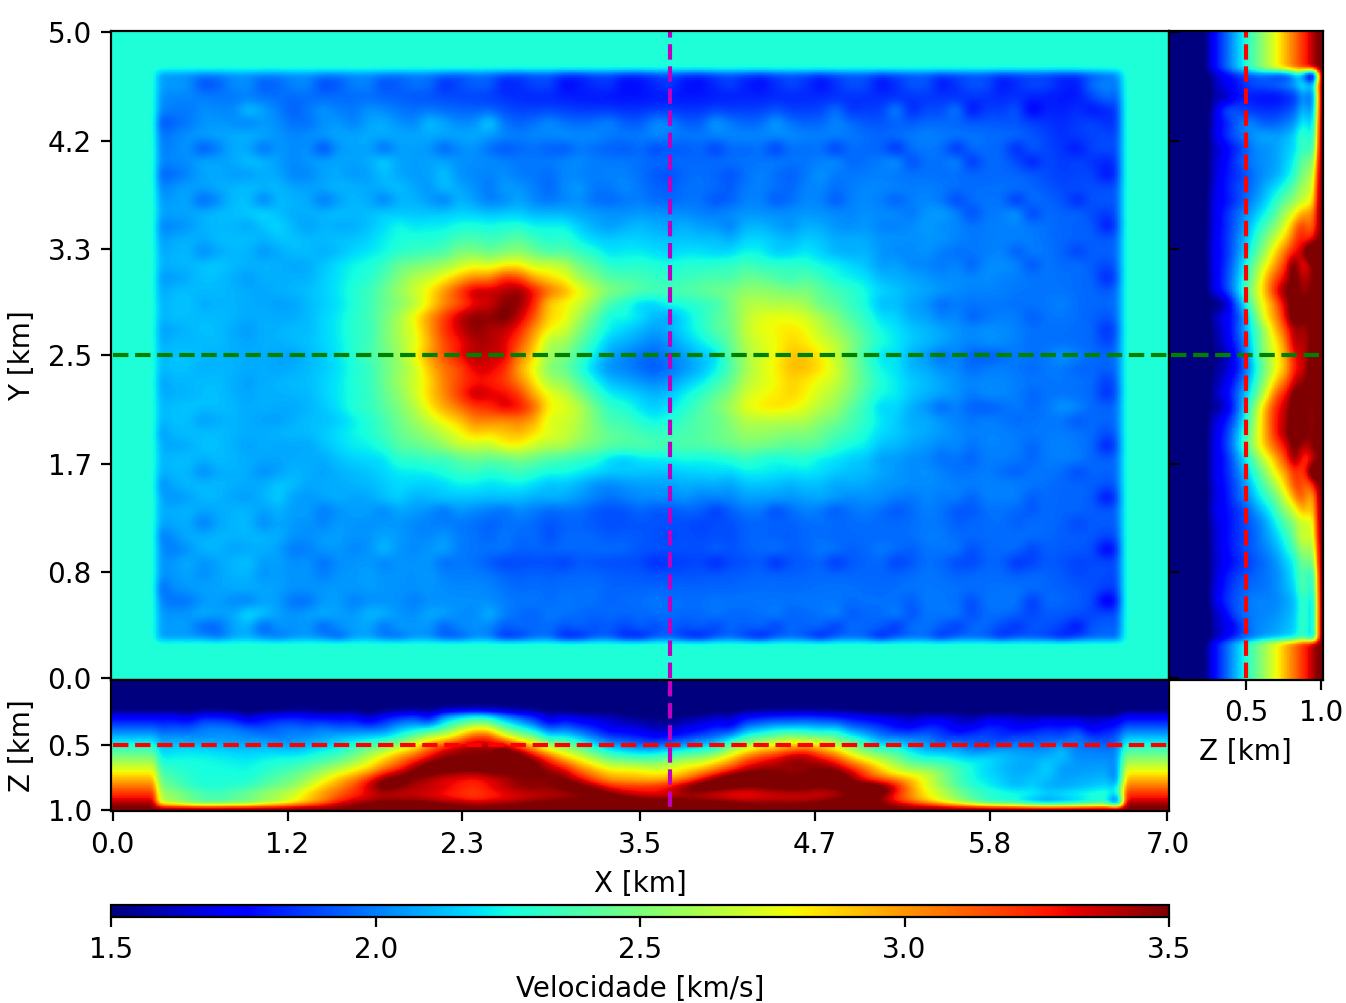
\includegraphics[width=12cm,height=9cm]{Imgs/Resultados/fim_refined.png}
	\caption{Modelo recuperado utilizando o \textit{Fast Iterative Method} em malha refinada.}
	\label{fig:fim_refined}	
\end{figure}

\begin{figure}[H]
	\centering
	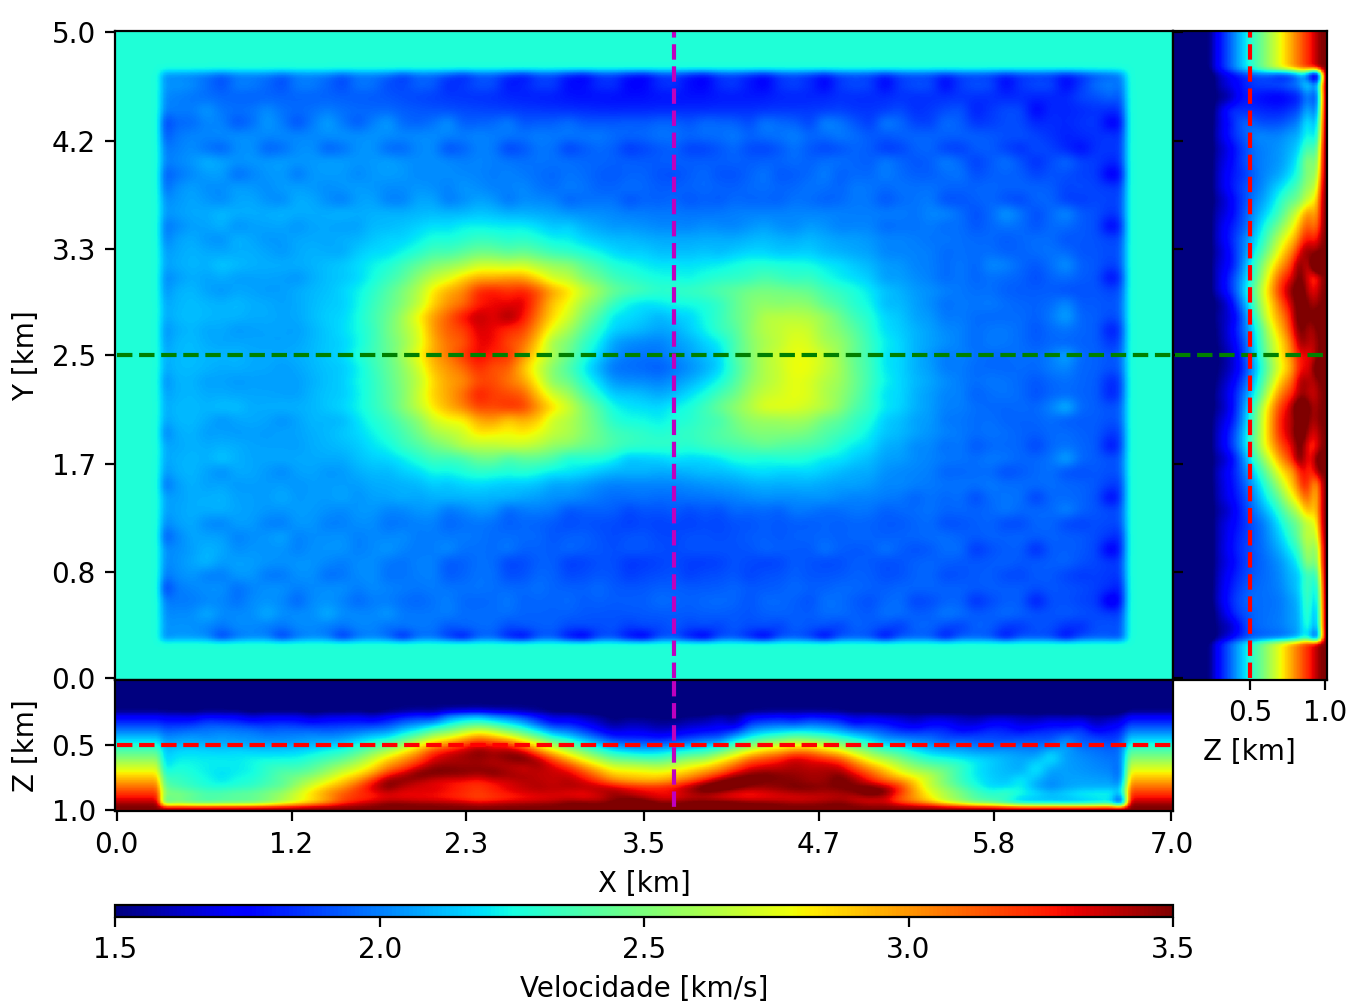
\includegraphics[width=12cm,height=9cm]{Imgs/Resultados/fsm_refined.png}
	\caption{Modelo recuperado utilizando \textit{Fast Sweeping Method} em malha refinada.}
	\label{fig:fsm_refined}	
\end{figure}
